% Esquema de difusión: el mismo controlador cierra dos lazos, uno con la planta
% simulada y otro con el modelo identificado, y se comparan las dos respuestas.
% Compilar con XeLaTeX.
\documentclass[border=8pt]{standalone}
\usepackage{fontspec}
\IfFontExistsTF{Arial}{\setmainfont{Arial}}{\setmainfont{TeX Gyre Heros}}
\usepackage{tikz}
\usetikzlibrary{arrows.meta,positioning,calc}
\definecolor{azul}{HTML}{1F5F99}
\definecolor{naranja}{HTML}{C8590E}
\definecolor{gris}{HTML}{5C5C58}
\begin{document}
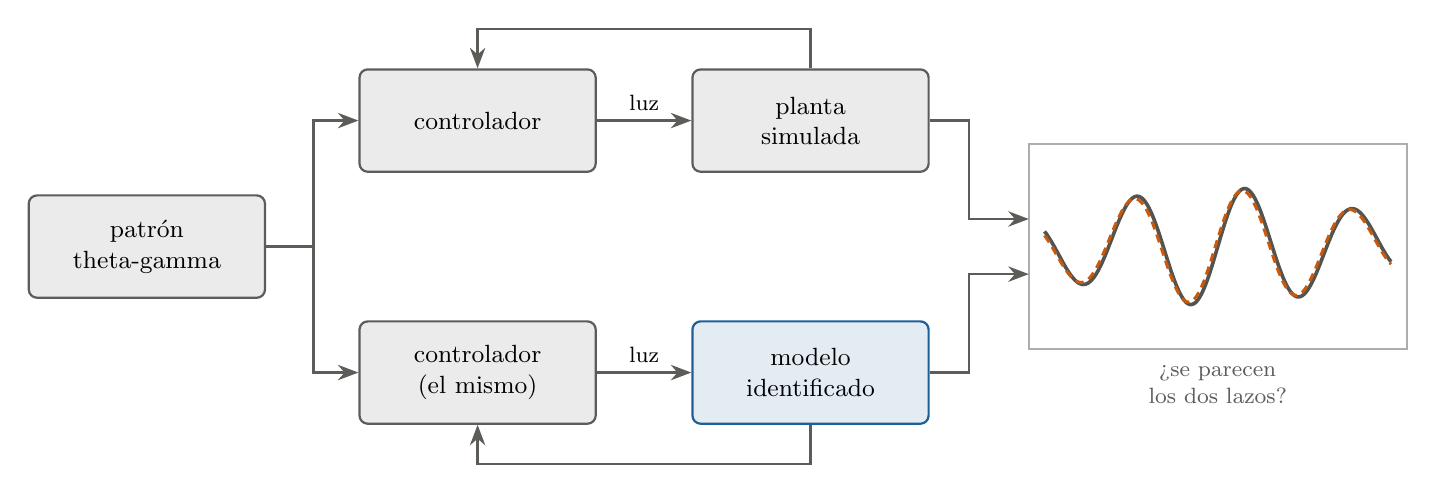
\begin{tikzpicture}[font=\small,
  caja/.style={draw=#1, fill=#1!12, rounded corners=3pt, align=center, inner sep=5pt,
               minimum width=30mm, minimum height=13mm, line width=0.8pt},
  flecha/.style={-{Stealth[length=2.6mm]}, line width=0.9pt, draw=gris}]

\node[caja=gris] (ref) at (0,0) {patrón\\theta-gamma};

\node[caja=gris] (c1) at (4.2,1.6) {controlador};
\node[caja=gris, right=12mm of c1] (p1) {planta\\simulada};
\node[caja=gris] (c2) at (4.2,-1.6) {controlador\\(el mismo)};
\node[caja=azul, right=12mm of c2] (p2) {modelo\\identificado};

\draw[flecha] (ref.east) -- ++(6mm,0) |- (c1.west);
\draw[flecha] (ref.east) -- ++(6mm,0) |- (c2.west);
\draw[flecha] (c1) -- node[above, font=\footnotesize] {luz} (p1);
\draw[flecha] (c2) -- node[above, font=\footnotesize] {luz} (p2);
\draw[flecha] (p1.north) -- ++(0,5mm) -| (c1.north);
\draw[flecha] (p2.south) -- ++(0,-5mm) -| (c2.south);

% respuestas superpuestas: el criterio es que los dos lazos se parezcan
\begin{scope}[shift={(13.6,0)}]
  \draw[gris!50, line width=0.6pt] (-2.4,-1.3) rectangle (2.4,1.3);
  \draw[gris!90!black, line width=1.3pt, domain=-2.2:2.2, samples=200, smooth]
    plot (\x, {0.75*sin(260*\x)*exp(-0.15*\x*\x)});
  \draw[naranja, line width=1.1pt, dash pattern=on 3pt off 2pt, domain=-2.2:2.2, samples=200, smooth]
    plot (\x, {0.72*sin(260*\x+8)*exp(-0.15*\x*\x)});
  \node[font=\footnotesize, align=center, text=gris] at (0,-1.75) {¿se parecen\\los dos lazos?};
\end{scope}
\draw[flecha] (p1.east) -- ++(5mm,0) |- (11.2,0.35);
\draw[flecha] (p2.east) -- ++(5mm,0) |- (11.2,-0.35);
\end{tikzpicture}
\end{document}
